

\section{Results}
\label{sec:results}

\begin{table}[h]
	\scriptsize
	\centering
	\begin{tabular}{l|cccccccc}
		\toprule[1pt]
		& \multicolumn{2}{l}{\makecell[c]{\textbf{Dialogue}\\\textbf{Summarization}}}& \multicolumn{2}{c}{\makecell[c]{\textbf{Question}\\\textbf{Generation}}}
		& \multicolumn{2}{c}{\makecell[c]{\textbf{Reading}\\\textbf{Comprehension}}}  \\
		
		{\textbf{Approach}}  & \textbf{R2} & \textbf{BertS} & \textbf{Bleu} & \textbf{RL} & \textbf{Bleu} & \textbf{RL}\\
		\hline
		Vanilla & 28.12 &  75.09 & 18.57 & 56.04& 28.42&73.33  \\
		Emb & 28.12 & 75.14 & 19.97 & 56.83 & 26.35 & 69.31 \\
		Aug  & 28.29 &  75.26 & 18.53 & 55.56&27.09 & 71.88 \\
		
		
		%Cross & \\
		Ins$\star$  & \textbf{28.97} & \textbf{75.63} & \textbf{20.26} & \textbf{56.85} & \textbf{29.44} & \textbf{74.03}\\	
		
		
		\bottomrule[1pt]
	\end{tabular}
	\caption{Performances(\%) of offline approaches on the original test set. Vanilla refers to the baseline that simply fine-tuned the basic pre-trained model on the original dataset for different tasks. $\star$ marks our approach.}
	\label{tab:mdresults-vanilla}
\end{table}


We show performances of approaches first, followed by ablation studies and human evaluations.
Then, we take a closer look at offline approaches, which show the inherent capability of models, with multi-faceted analysis. Hyper-parameter search and case studies are in Appendixes.%performing on different groups of people. 
%\footnote{Since we mainly focus on the differences of generation results which can be easily reflected by evaluation metrics, we didn't carry out human evaluations in this work.}
%At last, we show the  of our approach. %do ablation studies of our approach in the aspect of hyper-parameter search.


\subsection{Performance of Offline Approaches}
\label{sec:mda}
% original test set, in-distribution test set, all names test set





% It improves R2 with 0.17\% which is not consistent with the 0.40\% improvements in~\citet{liu2021controllable}. We think this is mainly due to the stochastic sampling operation of doing data augmentation.
%Our results are more reliable, since the results in our work are averaged over three times with training data augmented with different random seeds while \citet{liu2021controllable} didn't mention how many runs they took. 

\begin{table}[t]
	\scriptsize
	\centering
	\begin{subtable}{\linewidth}
		\scriptsize
		\centering
		\begin{tabular}{p{0.9cm}|p{0.36cm}p{0.36cm}p{0.36cm}p{0.36cm}|p{0.36cm}p{0.36cm}p{0.36cm}p{0.38cm}}
			\toprule[1pt]
		%	\textbf{Approach} & \textbf{R2} & \textbf{BertS} & \textbf{D-R2} & \textbf{R-R2} & \textbf{D-BertS} & \textbf{R-BertS}  \\
			& \multicolumn{4}{c|}{\textbf{R2}} & \multicolumn{4}{c}{\textbf{BertScore}} \\
			 %\cline{2-9}
			\textbf{Approach}& - & S$\downarrow$  & R$\downarrow$ & D$\downarrow$& - & S$\downarrow$ & R$\downarrow$& D$\downarrow$  \\
			
			
			\hline
			\multicolumn{9}{l}{\textit{In-distribution Names}}\\
			Vanilla & 27.66 & 31.24  & 13.98 & 5.51 &74.90&11.80&6.41& 2.49\\
			Emb & 27.63 & 29.39& 13.21 & 5.20 &74.91 &11.29 & 6.26& 2.43 \\
			Aug & 27.82 &27.35  & 12.33 & 4.86&74.95& 10.42 & 5.77 &2.57 \\
			

			%Cross & \\
			Ins$\star$  &  \underline{\textbf{28.79}} & \underline{\textbf{21.36}} & \underline{\textbf{9.50}} & \underline{\textbf{3.82}}& \textbf{75.48}&\underline{\textbf{7.94}} & \underline{\textbf{4.32}}& \underline{\textbf{1.71}} \\
			
			\hline
			\multicolumn{9}{l}{\textit{All-possible Names}}\\
			Vanilla & 27.19 & 33.10& 14.64 & 5.72 &74.83&12.26 & 6.66 & 2.60\\
			Emb & 27.22 & 31.38 & 13.59 & 5.30&74.89 &12.03 & 6.63 & 2.55\\
			Aug &27.50 &28.17 & 12.56 & 4.97 &74.96 &10.56 & 5.76 & 2.25 \\
			

			%Cross & \\
			Ins$\star$  &  \underline{\textbf{28.44}} & \underline{\textbf{25.37}}  & \textbf{11.58} & \textbf{4.62}&\textbf{75.38} &\underline{\textbf{9.38}} & \textbf{5.22}& \textbf{2.05} \\
			
			\bottomrule[1pt]
		\end{tabular}
		\caption{Dialogue Summarization}
		\label{tab:mdresults-ds}
	\end{subtable}
	
	\begin{subtable}{\linewidth}
		\scriptsize
		\centering
		\begin{tabular}{p{0.9cm}|p{0.36cm}p{0.36cm}p{0.36cm}p{0.36cm}|p{0.36cm}p{0.36cm}p{0.36cm}p{0.38cm}}
			\toprule[1pt]
			
			%\textbf{Approach} & \textbf{Bleu} & \textbf{RL} & \textbf{D-Bleu} & \textbf{R-Bleu} & \textbf{D-RL} & \textbf{R-RL}  \\
			 & \multicolumn{4}{c|}{\textbf{Bleu}} & \multicolumn{4}{c}{\textbf{RL}} \\
			%\cline{2-9}
			\textbf{Approach}& - & S$\downarrow$ & R$\downarrow$ & D$\downarrow$ & - & S$\downarrow$ & R$\downarrow$ & D$\downarrow$ \\
			
			\hline
			\multicolumn{9}{l}{\textit{In-distribution Names}}\\
			Vanilla & 18.48 &  34.80& 11.96 & 5.06&{57.14}&14.94&14.19 & 5.74\\
			Emb & 19.00 &38.24& 13.76 & 5.79 & 57.31 &17.55& 16.85 & 6.82 \\
			Aug & 17.89 & 26.24  & 8.22& {3.52}&56.26& 12.04& {11.35} & {4.69} \\
			

			%Cross & \\
			Ins$\star$ &  \textbf{19.58 }&\underline{\textbf{16.90}} & \underline{\textbf{5.53}} & \underline{\textbf{2.35}}& \textbf{57.47} &\underline{\textbf{7.83}} & \underline{\textbf{8.09}} &\underline{\textbf{3.35}}\\

			
			\hline
			\multicolumn{9}{l}{\textit{All-possible Names}}\\
			Vanilla & 18.56 & 29.64 & 10.04 & 4.26& {57.38}&12.98& 11.88 & 4.90 \\
			Emb & 18.70 & 35.52& 12.55 & 5.27 &57.28 &16.05 & 15.26 & 6.20 \\
			Aug & 17.81 &  23.09 & {7.15} & {3.06}&56.08&10.66& {9.64} & {4.03} \\
			

			%Cross & \\
			Ins$\star$ &  \textbf{19.57} & \underline{\textbf{14.65}} & \underline{\textbf{4.41}} & \underline{\textbf{1.90}} &\textbf{57.49}&\underline{\textbf{6.96}} & \underline{\textbf{6.58}} & \underline{\textbf{2.78}}\\
			
			\bottomrule[1pt]
		\end{tabular}
		\caption{Question Generation}
		\label{tab:mdresults-qg}
	\end{subtable}
	
	\begin{subtable}{\linewidth}
		\scriptsize
		\centering
		\begin{tabular}{p{0.9cm}|p{0.36cm}p{0.36cm}p{0.36cm}p{0.36cm}|p{0.36cm}p{0.36cm}p{0.36cm}p{0.38cm}}
			\toprule[1pt]
			%\textbf{Approach} & \textbf{Bleu} & \textbf{RL} & \textbf{D-Bleu} & \textbf{R-Bleu} & \textbf{D-RL} & \textbf{R-RL} \\
			& \multicolumn{4}{c|}{\textbf{BLEU}} & \multicolumn{4}{c}{\textbf{RL}} \\
			%\cline{2-9}
			\textbf{Approach}& - & S$\downarrow$ & R$\downarrow$& D$\downarrow$  & - & S$\downarrow$  & R$\downarrow$& D$\downarrow$ \\
			\hline
			\multicolumn{9}{l}{\textit{In-distribution Names}}\\
			Vanilla &28.34 & 54.98 & 6.54 & 2.83 &73.07&7.54& 9.69 & 4.17 \\
			Emb & 25.80 &57.78& 7.17 & 3.13 & 69.29 &9.83& 12.30 & 5.31 \\
			Aug & 27.07 & 55.96& 6.04 & 2.62 & 72.11&8.14 & 10.42&  4.50 \\
			

			Ins$\star$ & \underline{\textbf{29.31}} &\underline{\textbf{52.03}}& \underline{\textbf{4.53}} & \underline{\textbf{1.97}} & \textbf{74.04} &\underline{\textbf{5.65}} & \underline{\textbf{7.66}} & \underline{\textbf{3.32}}\\
			
			\hline
			\multicolumn{9}{l}{\textit{All-possible Names}}\\
			Vanilla &  28.56 & 53.94& 5.39 & 2.34& 73.60&6.39 & 8.21  & 3.53\\
			Emb &25.99 &  56.22 & 5.11 & 2.21&69.59&7.29 & 8.60 & 3.69\\
			Aug & 27.12 & 54.72 & 5.15 & 2.23& 72.23& 6.39 & 8.29  & 3.58\\
			
			Ins$\star$ &  \underline{\textbf{29.34}} &\underline{\textbf{51.38}}  & \underline{\textbf{3.66}} & \underline{\textbf{1.59}}& \textbf{74.35}&\underline{\textbf{4.62}} & \underline{\textbf{6.15}} & \underline{\textbf{2.64}}\\
			
			\bottomrule[1pt]
		\end{tabular}
		\caption{Reading Comprehension}
		\label{tab:mdresults-rc}
	\end{subtable}
	\caption{Performances(\%) of offline approaches. ``-'' is the original metric. S, D and R are shorted for the sensitivity metrics. Scores significantly better than all the baselines with p-value$<$0.05 are underlined.}	
	\label{tab:mdresults-main}
\end{table}

The performance on the original test sets is shown in Table~\ref{tab:mdresults-vanilla}. Emb only outperforms Vanilla on question generation and Aug only makes little improvements over Vanilla on dialogue summarization. %and even drops on the other two tasks.
Our approach {Ins} makes consistent improvements, {performing best among offline approaches}.

Results with sensitivity scores are in Table~\ref{tab:mdresults-main}. 
Emb fails to generate more insensitive results, especially for question generation.
{Aug} doesn't make promising improvements on outputs' quality over Vanilla, but it {reduces the sensitiveness of models} across different test sets and tasks.
Ins leads to better results on randomly augmented training data with different random seeds, significantly outperforming Aug. %with p-value<0.05.
In a word, Ins achieves the best performance among offline approaches. %, achieving the state-of-the-art results}.

By comparing the results in Table~\ref{tab:mdresults-main} horizontally, in-distribution names perform better than all-possible names on dialogue summarization, whereas results are opposite on the others. Speaker names in SAMSum are mostly real and popular names, while names in Molweni are online nicknames containing unknown words, such as ``zykotick9''. All-possible names contain a large proportion of real names, and a small proportion of names never seen during pre-training which can be regarded as nicknames. In this way, we can observe that the difficulty of modeling names for a model is ``SAMSum in-distribution  $<$ all-possible $<$ Molweni in-distribution''. In other words, models perform better on more popular names, which is in accord with the success of Fre in Sec.~\ref{sec:onlineapproach}.









\subsection{Performance of Online Approaches}
\label{sec:onlineapproach}
% replaced test set

The results of online approaches are in Table~\ref{tab:ddresults-main}.


\begin{table}[h]
	\scriptsize
	\centering
	\begin{subtable}{\linewidth}
		\scriptsize
		\centering
		\begin{tabular}{p{0.9cm}|p{0.36cm}p{0.36cm}p{0.36cm}p{0.36cm}|p{0.36cm}p{0.36cm}p{0.36cm}p{0.38cm}}
			\toprule[1pt]
			
			%\textbf{Approach} & \textbf{Bleu} & \textbf{RL} & \textbf{D-Bleu} & \textbf{R-Bleu} & \textbf{D-RL} & \textbf{R-RL}  \\
			
			 & \multicolumn{4}{c|}{\textbf{R2}} & \multicolumn{4}{c}{\textbf{BertScore}} \\
			%\cline{2-9}
			\textbf{Approach}& - & S$\downarrow$  & R$\downarrow$ & D$\downarrow$& - & S$\downarrow$  & R$\downarrow$& D$\downarrow$ \\
			\hline
			%Vanilla & 28.12 & 75.09 & - &-&-&-\\
			ID & 26.97 & - & - &-&74.26&-&-&-\\
			Fre & {28.55} & 25.17 & 11.31 & 4.50 &74.24&9.77 & 5.30 & 2.09 \\
			FreAug & 27.86 & 25.03 & {11.09} & {4.39}&75.02 &9.58 & {5.12}& 2.02 \\
			
			FreIns$\star$ & \underline{\textbf{28.73}} &\underline{\textbf{17.25}} & \underline{\textbf{7.66}} & \underline{\textbf{3.14}}& \underline{\textbf{75.53}}&\underline{\textbf{6.39}}& \underline{\textbf{3.43}} & \underline{\textbf{1.38}} \\
			\bottomrule[1pt]
		\end{tabular}
		\caption{Dialogue Summarization}
		\label{tab:ddresults-ds}
	\end{subtable}
	
	\begin{subtable}{\linewidth}
		\scriptsize
		\centering
		\begin{tabular}{p{0.9cm}|p{0.36cm}p{0.36cm}p{0.36cm}p{0.36cm}|p{0.36cm}p{0.36cm}p{0.36cm}p{0.36cm}}
			\toprule[1pt]
			%\textbf{Approach} & \textbf{Bleu} & \textbf{RL} & \textbf{D-Bleu} & \textbf{R-Bleu}& \textbf{D-RL} & \textbf{R-RL}  \\
			 & \multicolumn{4}{c|}{\textbf{BLEU}} & \multicolumn{4}{c}{\textbf{RL}} \\
			%\cline{2-9}
			\textbf{Approach}& - & S$\downarrow$ & R$\downarrow$ & D$\downarrow$ & - & S$\downarrow$  & R$\downarrow$& D$\downarrow$ \\
			\hline
			%Vanilla & 18.57 & 56.40 & - &-&-&-\\
			ID & {19.21} & - & - &-&56.49&-&-&-\\
			Fre & {18.96} & 18.44  & 5.51 & 2.35&{57.10}&8.35& 7.23  & 3.04 \\
			FreAug &  18.52 & 16.01& 4.92 & 2.14& 57.06 & 7.05& 6.50& 2.76 \\
			FreIns$\star$ & \textbf{19.71} &\underline{\textbf{10.09}} & \underline{\textbf{3.12}} & \underline{\textbf{1.35}}& \textbf{57.29} &\underline{\textbf{4.48}} & \underline{\textbf{4.19}} & \underline{\textbf{1.80}}\\
			\bottomrule[1pt]
		\end{tabular}
		\caption{Question Generation}
		\label{tab:ddresults-qg}
	\end{subtable}
	
	\begin{subtable}{\linewidth}
		\scriptsize
		\centering
		\begin{tabular}{p{0.9cm}|p{0.36cm}p{0.36cm}p{0.36cm}p{0.36cm}|p{0.36cm}p{0.36cm}p{0.36cm}p{0.36cm}}
			\toprule[1pt]
			%\textbf{Approach} & \textbf{Bleu} & \textbf{RL} & \textbf{D-Bleu} & \textbf{R-Bleu} & \textbf{D-RL} & \textbf{R-RL} \\
			& \multicolumn{4}{c|}{\textbf{BLEU}} & \multicolumn{4}{c}{\textbf{RL}} \\
			%\cline{2-9}
			\textbf{Approach}& - & S$\downarrow$  & R$\downarrow$ & D$\downarrow$& - & S$\downarrow$  & R$\downarrow$ & D$\downarrow$\\
			\hline
			%Vanilla & 28.42 & 73.33 & - &-&-&-\\
			ID & 28.46 & - & - &-&73.62&-&-&-\\
			Fre & 27.35 & 54.55& 3.77 & 1.63& 73.56 &4.95& 6.05 & 2.61  \\
			FreAug & 27.92 & 52.67 & 3.28& 1.42 &73.67&4.24& 5.63& 2.43  \\
			FreIns$\star$ &  \textbf{29.03} &\textbf{52.28}  & \textbf{2.66}& \textbf{1.15}& \textbf{74.59}&\underline{\textbf{3.28}}  & \underline{\textbf{4.51}}& \underline{\textbf{1.95}}\\
			\bottomrule[1pt]
		\end{tabular}
		\caption{Reading Comprehension}
		\label{tab:ddresults-rc}
	\end{subtable}
	\caption{Performances(\%) of online approaches.}%Scores significantly better than the baselines with p-value$<$0.05 are underlined. }	
	\label{tab:ddresults-main}
\end{table}




All speaker names will be normalized into fixed code names in {ID}, so that the test set for ID is changeless for each sample and the sensitivity scores are actually 0.0. Unfortunately, its quality scores lag behind Ins and even drop dramatically on dialogue summarization. Thus, it's not recommended to be a necessary data pre-processing step.  % The differences among code names is only a number, making them more indistinguishable by models. Moreover,  % However, comparing the quality metrics with other approaches, the  % Some latent but important characteristics in names are neglected such as gender.

{Fre} makes some improvements on R2 for dialogue summarization by comparing with the vanilla model, which is consistent with the results in~\cite{khalifa2021bag}, whereas the drops in BertScore were not mentioned in their work. The sensitivity scores are lower than those for offline approaches in Table~\ref{tab:mdresults-main}. To better understand the gains of Fre, we further test the vanilla model with the same test sets replaced by frequent names. It achieves similar performance on Rouge-2 (28.18) and BertScore (75.13) with the vanilla model. The sensitivity score D-BertS is 2.24, which is lower than 2.49 of Vanilla in Table~\ref{tab:mdresults-main}. It shows that {the advantages of Fre not only come from using the group of frequent names} that are easier for a model to understand, {but also from doing fine-tuning with this group of names}. FreAug doesn't improve the outputs' quality consistently, but reduces the sensitivity scores. %This is the same as the comparisons between Aug and Vanilla. 

{FreIns} performs the most insensitively with better generation quality among online approaches.


\subsection{Ablation Study}

Ablation studies of our full approach Ins are in Table~\ref{tab:ablation}.
Aug is regarded as an ablation representing the model trained without any auxiliary losses.
Both insensitivity losses outperform Aug with using $\mathcal{L}_{dh}$ topping the rank on most metrics, showing that penalizing differences on the decoder hidden states has more direct effects on the outputs.
Combining both losses induces more performance gains.

% DH and CA refer to the model trained only with $\mathcal{L}_{ca}$ or $\mathcal{L}_{dh}$ respectively, and 

\begin{table}[th]
	\scriptsize
	\centering
	\begin{tabular}{p{0.99cm}|p{0.3cm}cp{0.3cm}cp{0.3cm}c}
		\toprule[1pt]
		& \multicolumn{2}{l}{\makecell[c]{\textbf{Dialogue}\\\textbf{Summarization}}}& \multicolumn{2}{c}{\makecell[c]{\textbf{Question}\\\textbf{Generation}}}
		& \multicolumn{2}{c}{\makecell[c]{\textbf{Reading}\\\textbf{Comprehension}}}  \\
		{\textbf{Approach}}  & \textbf{BertS} & \textbf{D-BertS$\downarrow$} & \textbf{Bleu} & \textbf{D-Bleu$\downarrow$} & \textbf{Bleu} & \textbf{D-Bleu$\downarrow$}\\
		\hline
		Ins & \textbf{75.48} & \textbf{1.71} & 19.48 & \textbf{2.35} & \textbf{29.31} & \textbf{1.97} \\
		-w/o $\mathcal{L}_{ca}$ & 75.43 & 1.85 & \textbf{19.71} & 2.47 & 29.03 & 2.19 \\
		-w/o $\mathcal{L}_{dh}$& 74.89 & 2.27 & 18.40 & 3.01 & 28.42 & 2.04 \\
		Aug& 74.95 & 2.57 & 17.89 & 3.52 & 27.07 & 2.62 \\
		
		\bottomrule[1pt]
	\end{tabular}
	\caption{Ablations(\%) of the full approach Ins.}%with the in-distribution test setting.}
	\label{tab:ablation}
\end{table}

\subsection{Human Evaluation}

Taking dialogue summarization as an example, we did human evaluation to further prove the improvement on sensitivity by sampling 200 pairs of generations for each offline approach and asked three proficient English speakers to label each case out of 4 choices by selecting the primary one that makes the generations distinct: %  distinguishing one out of 4 choices:
%among 4 choices by choosing the major one that makes generations distinct: 
\textbf{Infor}mation difference means both outputs contain different information or keywords. 
\textbf{Fact}ual difference refers to different matchings between speakers and events.
%\textbf{Spea}ker reorder represents different orders of juxtaposed names.
\textbf{Expre}ssion difference is outputs having minor differences, such as capitalization and different orders of juxtaposed names.
\textbf{Same} represents the identical outputs.
The results are in Fig.~\ref{fig:humaneval} with 0.64 Kappa score, indicating substantial agreement. We can see that content distinction is the primary difference type. Ins generates less distinct contents and more identical results, outperforming the baselines.

\begin{figure}[t]
	\centering
	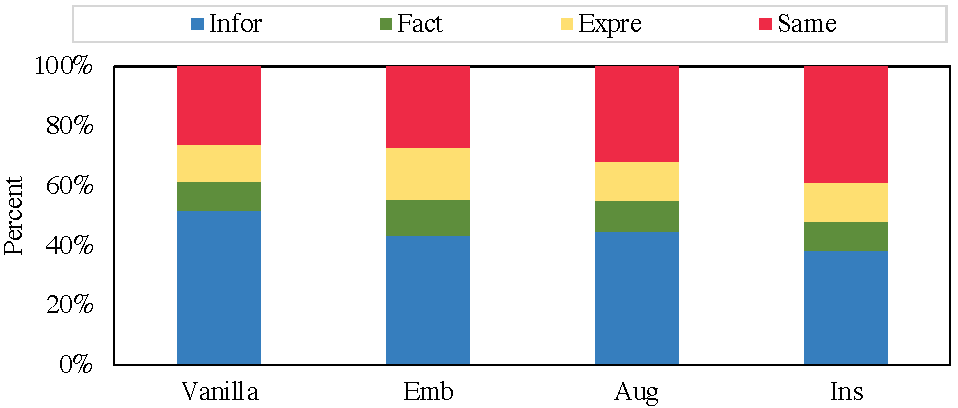
\includegraphics[width=0.9\columnwidth]{humaneval.pdf}
	\caption{Human evaluation for difference types.} %in the summaries.}
	%\underline{Divergent contents} are underlined in the generated summaries.}
	\label{fig:humaneval}
\end{figure}



\subsection{Sensitivity among Name Groups}
\label{sec:unfairness}
% divide by name occurance
We collect specific groups of names in terms of popularity and race and show differences in the quality performances on test sets constructed with corresponding names. 
%People from the same race are likely to have more communication. A severe ethical issue will show up if there exists unfairness among the different races. Although the popularity of names for speakers is stochastic for each dialogue, the model still has the potential facing dramatic performance drops caused by ``unpopular'' names from speakers who lead the dialogue. This may also accelerate the extinction of rare names, together with their cultures. 
%We illustrate the performances of different name groups under each approach 
%The results are illustrated in Fig.~\ref{fig:groups} and Figure~\ref{fig:groups2}. 
The sensitivity among different groups for each method are reflected by the scattering of dots vertically in Fig.~\ref{fig:groups}.% and Fig.~\ref{fig:groups2}. %Task-specific metrics on corresponding test sets show the fairness among groups, i.e. inter-group fairness. %The fairness within groups, i.e. intra-group fairness, is compared by sensitivity metrics.




%\begin{figure}[t]
%	\centering
%	\begin{minipage}[t]{\linewidth}
%		\centering
%		\subfloat[Dialogue Summarization]{
%			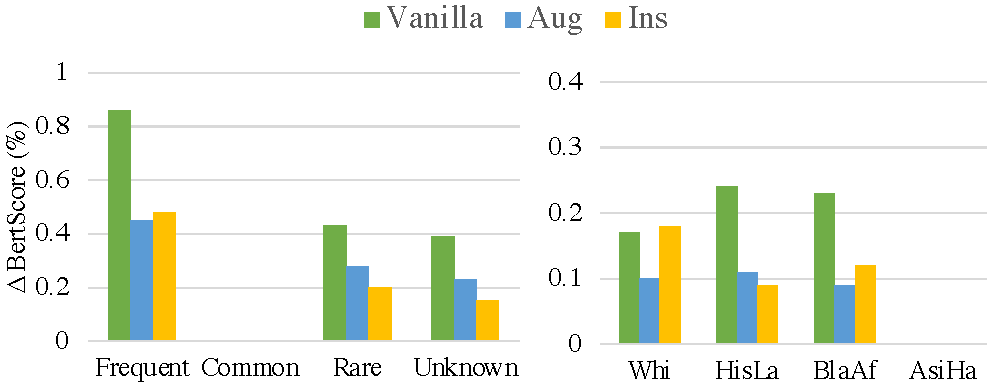
\includegraphics[scale=0.48]{samsum.pdf}
%			%\caption{fig1}
%		}%
%	\end{minipage}%
%	
%	\begin{minipage}[t]{\linewidth}
%		\centering
%		\subfloat[Question Generation]{
%			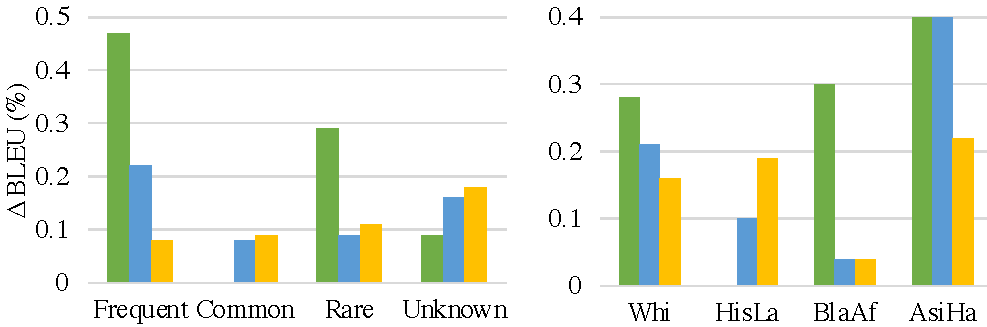
\includegraphics[scale=0.48]{molweni.pdf}
%			\label{fig:groups-mowelni}
%		}%
%	\end{minipage}
%	\centering
%	\caption{Unfairness among different groups of names.}	
%	\label{fig:groups}
%\end{figure}

%\label{sec:unfairnessstatistical}


\textbf{Name groups by popularity and usage:} We define 4 groups. \textbf{Frequent} including words frequently and solely used as human names is mentioned before. \textbf{Polysemous} represents words frequently used but not specialized for human names, such as June and Florida. \textbf{Rare} is names with low occurrence times like Paderau. \textbf{Unknown} names are similar to random strings from a model's perspective since they haven't been exposed to the model. The last three groups are collected by counting occurrences
of all-possible names in the pre-training corpus of BART. We select 200 names for each group (More details are in Appendix~\ref{sec:app-names}).
%100 males and 100 females for each group. 
%\JQ{polysemous}

According to Fig.~\ref{fig:groups-frequency}, we can see that models usually perform poorly on Polysemous, % for inter-group fairness, %and intra-group fairness, 
even worse than Rare and Unknown.  The daily meanings dominate the representation of this word and confuse the model. 
Frequent generally outperforms other groups.
%on both generation quality and on sensitivity scores. For example, R-BertS of the vanilla model tested with Frequent is only 5.70\%, which is not only significantly lower than other groups (Polysemous 7.79\%, Rare 6.69\%, Unknown 6.79\%), but also better than Vanilla with 6.41\% or 6.66\% in Table~\ref{tab:mdresults-main}. 
We conclude that 
words frequently and uniquely used as names that result in more specialized embeddings in pre-trained models and perform better. 
Moreover, comparing the sensitivity among different approaches, Ins outperforms the baselines in most cases except Aug. It achieves more centralized dots due to the performance reduction on the dominant groups or even all groups, showing that models tend to overfit with augmented data without our losses.
%When armed with our losses, the model understands the similarities and differences among augmented samples better and thus performs better with all groups
%Taking dialogue summarization in Fig.~\ref{fig:groups-frequency} as an example, Aug achieves more centralized dots mainly due to the performance decreases on the dominant groups, indicating that the model tends to overfit on these names. With the guidance of our losses, the model take better advantage of the augmented data  
To recap, Ins results in consistent improvements over Vanilla among different tasks compared with other baselines.
%Aug and Ins result in more fair performances. %with Ins topping the rank. 
% divide by racial




\begin{figure}[t]
	
	\begin{minipage}[t]{\linewidth}
		\centering
		\subfloat[Sensitivity among different popularity groups.]{
			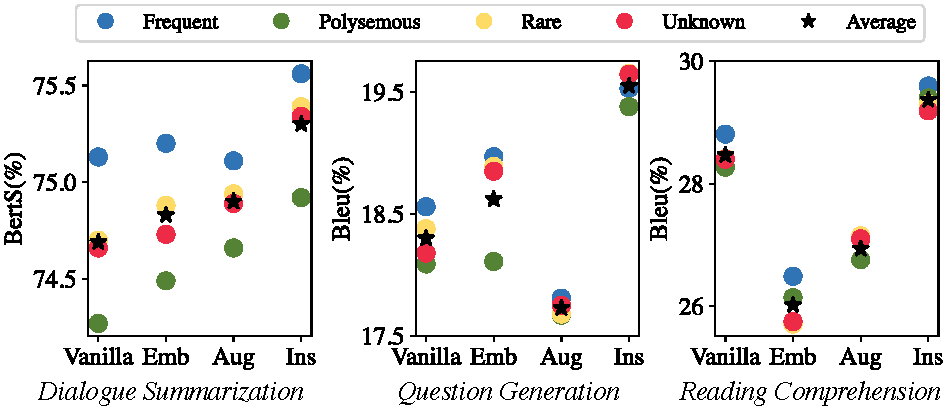
\includegraphics[scale=0.47]{frequency.pdf}
			\label{fig:groups-frequency}
			%\caption{fig1}
		}%
	\end{minipage}%
	
	\begin{minipage}[t]{\linewidth}
		\centering
		\subfloat[Sensitivity among different racial groups.]{
			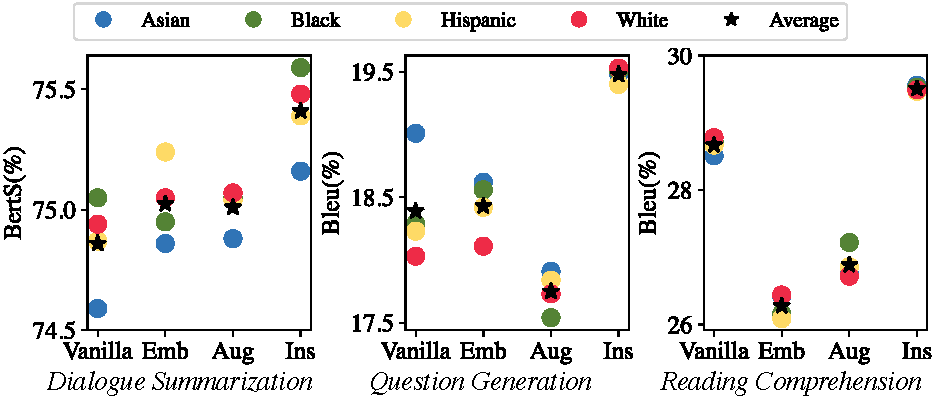
\includegraphics[scale=0.47]{racial.pdf}
			\label{fig:groups-racial}
		}%
	\end{minipage}
	\centering
	\caption{Sensitivity among names within different groups. The scores are the higher the better and more centralized dots for each approach represent better insensitivity among groups. }% The right figures shows intra-group fairness and the scores are expected to be lower.}	
	\label{fig:groups}
\end{figure}

\textbf{Name groups by races:} Names from different races are from~\citet{tzioumis2018demographic} by assigning each name to a race with the highest probability. 4 major groups\footnote{Other groups are empty after this assigning operation with \citet{tzioumis2018demographic}'s name list.} are gathered, including Non-Hispanic \textbf{White}, \textbf{Hispanic} or Latino, Non-Hispanic \textbf{Black} or African American, and Non-Hispanic \textbf{Asian} or Native Hawaiian or Other Pacific Islander. % containing 2,873, 424, 64 and 561 names respectively. 
To avoid the influence of the various number of names, we select the most frequent 50 names in each group and show the results in Fig.~\ref{fig:groups-racial}.
All of the approaches show discrimination against Asian in dialogue summarization. %according to inter-group results. %, and superiorities on White with lowest intra-group sensitivity. 
Emb, Aug and Ins improve the insensitivity among different races compared with Vanilla, and Ins is better with the guarantee on quality. We consider to introduce special designs on demographic features in the future.



%\begin{figure}[t]
	%\centering
	%\begin{minipage}[t]{\linewidth}
	%	\centering
	%	\subfloat[Dialogue Summarization]{
	%		\includegraphics[scale=0.5]{samsum-racial.pdf}
	%		%\caption{fig1}
	%	}%
	%\end{minipage}%
	%
	%\begin{minipage}[t]{\linewidth}
	%	\centering
	%	\subfloat[Question Generation]{
	%		\includegraphics[scale=0.5]{molweni-racial.pdf}
	%		\label{fig:groups-mowelni}
	%	}%
	%\end{minipage}
%	\centering
%	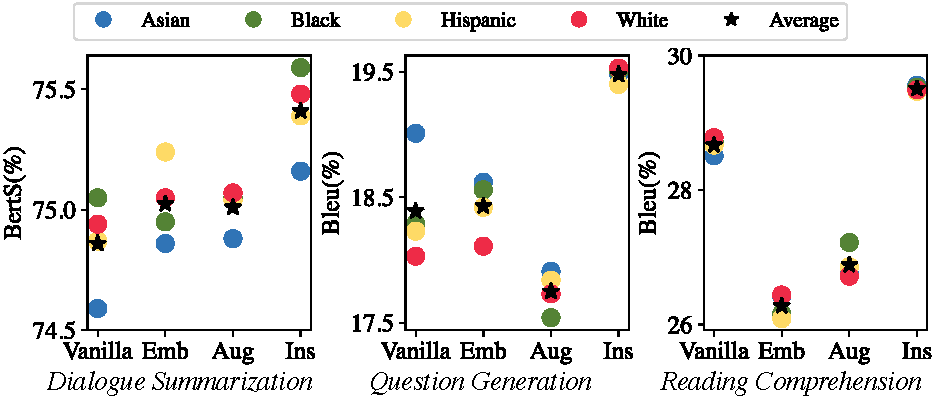
\includegraphics[scale=0.5]{racial.pdf}
%	\caption{Sensitivity among different racial groups.  }	
%	\label{fig:groups2}
%\end{figure}
\subsection{Sensitivity on an Individual Speaker}

We can also only change the name of a single speaker each time to analyze fine-grained sensitivity.
The results of offline approaches for dialogue summarization are shown in Table~\ref{tab: change-one-name} (see more in Appendix~\ref{sec:app-results}).
The sensitivity scores are lower than the ones in Table~\ref{tab:mdresults-main}. It seems that the sensitivity of models is proportional to the amount of changes in test samples, i.e., whether changing all speaker names (change-all-name) or only one speaker name (change-one-name). However,
%by analyzing the relations of sample-wise and speaker-wise sensitivity scores for each sample, 
it's not always true and changing one name can be more sensitive than changing all names. Taking the results from Ins as an example, around 52.01\% samples have speakers whose change-one-name D-BertS is higher than the corresponding changel-all-name one. Over 34.80\% of the change-one-name D-BertS averaged by speakers from the same dialogue is also higher than the change-all-name D-BertS. We further show the trends between speaker features and their sensitivity scores in Fig.~\ref{fig:trends}. Names are more sensitive and thus crucial for speakers at the start of a dialogue or with more utterances, deserving attention for further improvements. 


\begin{table}[]
	\scriptsize
	\centering
	\begin{tabular}{p{0.9cm}|p{0.36cm}p{0.36cm}p{0.36cm}p{0.36cm}|p{0.36cm}p{0.36cm}p{0.36cm}p{0.38cm}}
		\toprule[1pt]
		
		%\textbf{Approach} & \textbf{Bleu} & \textbf{RL} & \textbf{D-Bleu} & \textbf{R-Bleu} & \textbf{D-RL} & \textbf{R-RL}  \\
		
		 & \multicolumn{4}{c|}{\textbf{R2}} & \multicolumn{4}{c}{\textbf{BertScore}} \\
		%\cline{2-9}
		\textbf{Approach}& - & S$\downarrow$  & R$\downarrow$ & D$\downarrow$& - & S$\downarrow$  & R$\downarrow$& D$\downarrow$ \\
		\hline
		\multicolumn{7}{l}{\textit{In-distribution Names}}\\
		Vanilla & 27.29 &25.53 & 11.05& 4.42& 74.64 &9.65&5.19 & 2.05\\
		Emb & 27.41 &24.20 & 10.87 & 4.33& 74.90 &9.49 & 5.29& 2.09 \\
		Aug &
		{27.51} & 22.24 & {9.89} & {3.96} &74.83&8.50 & 4.67 & {1.85}\\
		Ins$\star$ & \textbf{28.70} &\underline{\textbf{16.54}}  & \textbf{7.19} & \textbf{2.92}& \textbf{75.44}&\underline{\textbf{6.11}}& \textbf{3.18}& \textbf{1.28} \\
		
		\hline
		\multicolumn{7}{l}{\textit{All-possible Names}}\\
		Vanilla &
		27.32& 23.77  & 11.07 & 4.45&74.81 &9.61 &5.15& 2.04  \\
		Emb & 27.26 & 24.98 & 10.68 & 4.25& 75.30&9.57 & 5.16& 2.02\\
		Aug  &
		27.36 & 22.73 & {10.04} & {4.03} &74.86&8.56 & 4.69 & 1.87\\
		Ins$\star$  & \textbf{28.38} &\underline{\textbf{18.65}} & \textbf{8.12}& \textbf{3.29}  &\textbf{75.35} &\underline{\textbf{6.89}}& \textbf{3.75} & \textbf{1.50} \\
		
		\bottomrule[1pt]
	\end{tabular}
	\caption{Dialogue summarization results(\%) of offline approaches for sensitivity on an individual speaker.}
	\label{tab: change-one-name}
\end{table}


\begin{figure}[h]
	\centering
	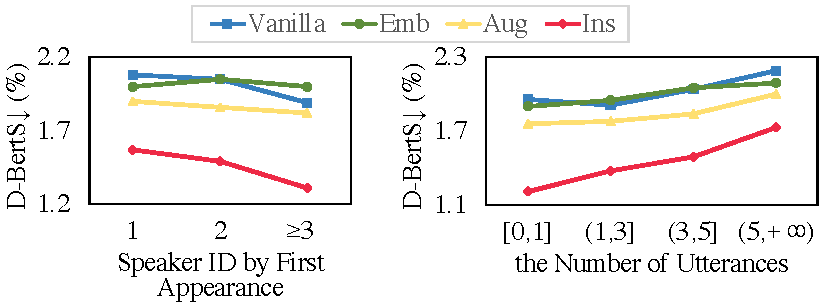
\includegraphics[scale=0.55]{speaker-sensitivity.pdf}
	
	\caption{Change-one-name sensitivities on different speaker features for dialogue summarization.}%with all-possible names
	\label{fig:trends}
\end{figure}



%This motivates us to analysis the possible factors causing sensitiveness in Section~\ref{sec:factors}.
% AugIns 57.88\% 38.95/%
% FreAugIns 56.65\%, 41.03\%




%\begin{table}[h]
%	\scriptsize
%	\centering
%	\begin{tabular}{crrrrr}
	%	\hline
	%	\textbf{Approach} & \textbf{Same} & \textbf{Cont} &\textbf{Spea} & \textbf{Reas}  & \textbf{Expre} \\
	%	\hline
	%	Vanilla &  &  & &  & \\
	%	Emb &  &  &  &  & \\
	%	Aug &  &  &  & & \\
	%	Ins &  &  &  &  & \\
	%	\hline
	%\end{tabular}
	%\caption{The percentage of different labels(\%).}
	%\label{tab:pilot}
%\end{table}



%\subsection{Hyper-parameter Search of Ins Loss}

%We search the hyper-parameter weight $\alpha$ from 0.7 to 0.9 with the intuition that our ins loss is an auxiliary training target and more attention still should be put on the vanilla loss. The results of Ins fine-tuned with different $\alpha$ on the original test set are shown in Figure~\ref{fig:hyperparameter}. We conclude that more weights should be put on $L_{ins}$ is for data containing rarer names. In this work, we set $0.9$ for dialogue summarization, $0.7$ and $0.9$ for Ins and FreIns respectively on question generation, and $0.8$ and $0.9$ for Ins and FreIns respectively on reading comprehension, by choosing the one performing best on $D_{va}$.
%\JQ{add conclusion: smaller alpha on datasets with more variant names}
%Our approach consistently outperforms Vanilla. 

%\begin{figure}[h]
%	\centering
%	\begin{minipage}[t]{0.5\linewidth}
%		\centering
%		\subfloat[Dialogue Summarization]{
%			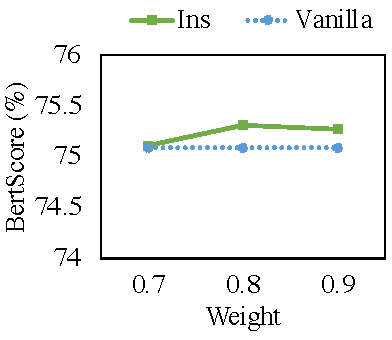
\includegraphics[scale=0.55]{samsum-weight.pdf}
			%\caption{fig1}
%		}%
%	\end{minipage}%
%	\begin{minipage}[t]{0.5\linewidth}
%		\centering
%		\subfloat[Question Generation]{
%			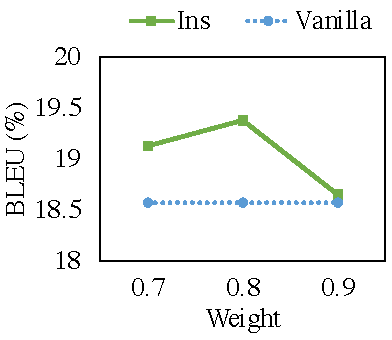
\includegraphics[scale=0.55]{molweni-weight.pdf}
			%\caption{fig2}
%		}%
%	\end{minipage}%
%	\centering
%	\caption{Results on the vanilla test sets of Ins with different weights.} %on the same augmented data  
%	\label{fig:hyperparameter}
%\end{figure}


%\subsection{Possible Factors for Speaker Sensitivity}
%\label{sec:factors}

%We analysis trends of speaker name sensitivity with different dialogue features in the granularity of both samples and speakers.
%In Figure~\ref{fig:trends} shows the results of AugIns's performances on all-possible names under different conditions. 
%The results are more volatile with dialogues having more speakers and more utterances according to the sample-wise sensitivity roughly. 
%The trends on speaker-wise sensitivity is more clear than that on sample-wise.
%Speakers showing up at the beginning of a dialogue and speaking more times have a larger influence on the results with different names, as they are likely to dominate the topic of the whole dialogue. In a word, the dominating speakers and dialogue complexity deserve attentions for further improvements.% 

%\begin{figure}[t]
%	\centering
%	\begin{minipage}[t]{\linewidth}
%		\centering
%		\subfloat[Sample-wise Sensitivity]{
%			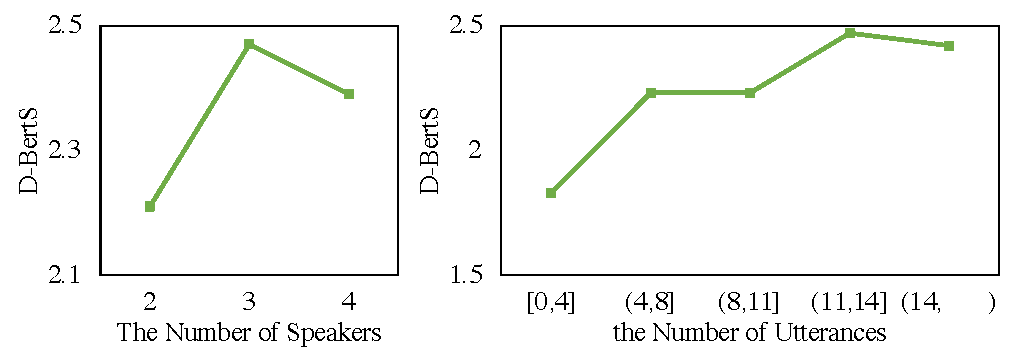
\includegraphics[scale=0.4]{sample-sensitivity.pdf}
%			%\caption{fig1}
%		}%
%	\end{minipage}%
%	
%	\begin{minipage}[t]{\linewidth}
%		\centering
%		\subfloat[Speaker-wise Sensitivity]{
%			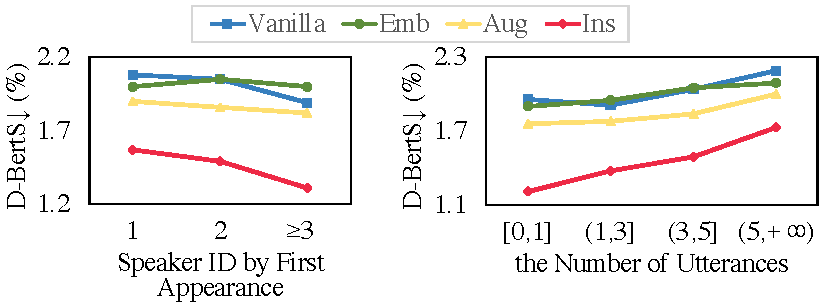
\includegraphics[scale=0.4]{speaker-sensitivity.pdf}
%			%\label{f}
%		}%
%	\end{minipage}
%	\centering
%	\caption{The trends of speaker name sensitivity with different dialogue features.}	
%	\label{fig:trends}
%\end{figure}



%\begin{table}[th]
%	\scriptsize
%	\centering
%	\begin{tabular}{crrrr}
%		\toprule[1pt]
%		& \multicolumn{2}{c}{Dialogue Sum.} & \multicolumn{2}{c}{Question Gen.} \\
%		{Weight}  & {R2} & {BertS} & Bleu & RL \\
%		\hline
		%0.6 &  28.11 & 75.24 & 18.80 & 56.23\\
%		vanilla & 28.12 & 75.09 & 18.57 & 56.04 \\
%		0.7  &  28.02 & 75.11 & 19.13* & 56.47*\\
%		0.8  &   28.03 & 75.31& 19.38 & 57.05\\
%		0.9 & 28.52* & 75.27* & 18.65& 56.10\\
%		\bottomrule[1pt]
%	\end{tabular}
%	\caption{Results on the corresponding vanilla test set of AugIns fine-tuned on the same augmented data with different weights.}
%	\label{tab:hyperparameter}
%\end{table}

%\subsection{Variants of Loss Design}